\chapter{Design}
\label{chap:design}

\section{System Sequence Diagram}
\begin{figure}[H]
	\centering
		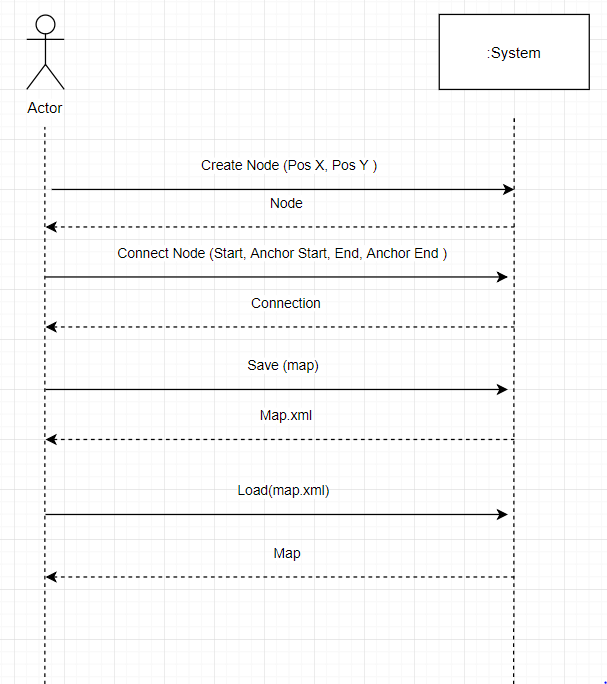
\includegraphics[scale=0.7]{images/SSD.png}
	\caption{System Sequence Diagramm}
	\label{fig:domain_model}
\end{figure}
\label{sec:system_sequence_diagram}
Wie beim Diagramm zu sehen ist, übergibt der Benutzer dem Programm
primär klicks auf bestimmte Objekte. Das Programm erstellt anhand der
Koordinaten dann so die Nodes und Connections. Beim Speicher Prozess 
erhält der Benutzer eine XML Datei mit den Informationen zu seinem Mindmap. Beim Lade Prozess übergibt der Benutzer dieses dann, dass Programm erstellt anhand der Informationen die Knoten auf der Map.


\section{UML Diagramme}
\label{sec:uml_diagramme}